\documentclass[11pt]{article}

\usepackage{float}
\usepackage{hyperref}
\usepackage{fullpage}
\usepackage{verbatim}
\usepackage{moreverb}
\usepackage{graphicx}
\usepackage{array}
\usepackage{booktabs}
\usepackage{parskip}
\usepackage{tikz}
\usetikzlibrary{arrows,automata, positioning}
\usepackage{minted}
\let\verbatiminput=\verbatimtabinput
\def\verbatimtabsize{4\relax}
\graphicspath{{images/}}

\begin{document}
\title{EECS 151/251A FPGA Lab\\
Lab 6: Multi-bit Clock-Crossing, FIFOs, UART Piano, Project Intro}

\author{Prof. Elad Alon \\
TAs: Vighnesh Iyer, Bob Zhou \\Department of Electrical Engineering and Computer Sciences\\
College of Engineering, University of California, Berkeley}
\date{}
\maketitle

\tableofcontents

\section{Intro}
In this lab, you will integrate the components you created in labs 4 and 5 (UART and AC97 controller). You will begin by building 2 varieties of FIFOs, asynchronous and synchronous, and verifying their functionality using a block-level testbench. You will then modify your AC97 controller to use a FIFO as its PCM data source. Finally, you will create some logic that integrates all these components to form a 'piano'.

Here is an overview of the entire system in \verb|ml505top| we are going to build. You may find it useful to refer to this block diagram while doing this lab.

\begin{figure}[H]
	\centerline{\includegraphics[width=\textwidth]{Lab6_Block_Diagram.png}}
\end{figure}

In this lab, you will be building the FIFOs, modifying your AC97 controller to use one, and designing the piano FSM. You will then construct a system-level testbench to verify functionality in simulation.

\section{Building a Synchronous FIFO}
A FIFO (first in, first out) data buffer is a circuit that has two interfaces: a read side and a write side. The FIFO we will build in this section will have both the read and write side clocked by the same clock; this circuit is known as a synchronous FIFO.

\subsection{FIFO Functionality}
A FIFO is implemented with a circular buffer (2D reg) and two pointers: a read pointer and a write pointer. These pointers address the buffer inside the FIFO, and they indicate where the next read or write operation should be performed. When the FIFO is reset, these pointers are set to the same value. 

When a write to the FIFO is performed, the write pointer increments and the data provided to the FIFO is written to the buffer. When a read from the FIFO is performed, the read pointer increments, and the data present at the read pointer's location is sent out of the FIFO.

A comparison between the values of the read and write pointers indicate whether the FIFO is full or empty. You can choose to implement this logic as you please. The \verb|Electronics| section of the \href{https://en.wikipedia.org/wiki/FIFO_(computing_and_electronics)}{FIFO Wikipedia article} will likely aid you in creating your FIFO.

Here is a block diagram of the FIFO you should create from page 103 of the \href{https://www.xilinx.com/support/documentation/ip_documentation/fifo_generator_ug175.pdf}{Xilinx FIFO IP Manual}.

\begin{center}
	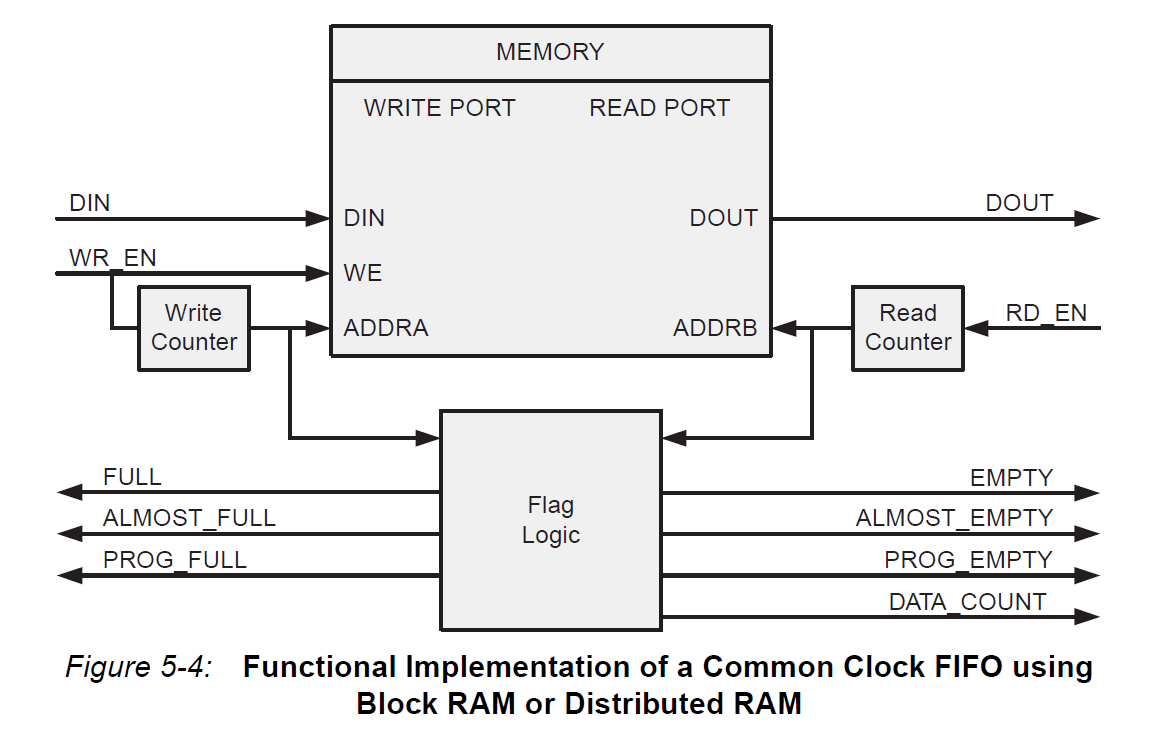
\includegraphics[height=7cm]{sync_fifo_diagram.png}
\end{center}

The interface of our FIFO will contain a subset of the signals enumerated in the diagram above.

\subsection{FIFO Interface}
Take a look at the FIFO skeleton in \verb|labs_sp17/lab6/src/fifo.v|.

Our FIFO is parameterized by these parameters:
\begin{itemize}
	\item \verb|data_width| - This parameter represents the number of bits per entry in the FIFO.
	\item \verb|fifo_depth| - This parameter represents the number of entries in the FIFO.
	\item \verb|addr_width| - This parameter is automatically filled by the log2 macro to be the number of bits for your read and write pointers.
\end{itemize}

The common FIFO signals are:
\begin{itemize}
	\item \verb|clk| - Clock used for both read and write interfaces of the FIFO.
	\item \verb|rst| - Reset synchronous to the clock; should cause the read and write pointers to be reset.
\end{itemize}

The FIFO write interface consists of three signals:
\begin{itemize}
	\item \verb|wr_en| - When this signal is high, on the rising edge of the clock, the data on \verb|din| will be written to the FIFO.
	\item \verb|[data_width-1:0] din| - The data to be written to the FIFO should be present on this net.
	\item \verb|full| - When this signal is high, it indicates that the FIFO is full.
\end{itemize}

The FIFO read interface consists of three signals:
\begin{itemize}
	\item \verb|rd_en| - When this signal is high, on the rising edge of the clock, the FIFO should present the data indexed by the write pointer on \verb|dout|
	\item \verb|[data_width-1:0] dout| - The data that was read from the FIFO after the rising edge on which \verb|rd_en| was asserted
	\item \verb|empty| - When this signal is high, it indicates that the FIFO is empty.
\end{itemize}

\subsection{FIFO Timing}
The FIFO that you design should conform to the specs above. To further, clarify here are the read and write timing diagrams from the \href{https://www.xilinx.com/support/documentation/ip_documentation/fifo_generator_ug175.pdf}{Xilinx FIFO IP Manual}. These diagrams can be found on pages 105 and 107. Your FIFO should behave similarly.

\begin{figure}[H]
	\minipage{0.48\textwidth}
	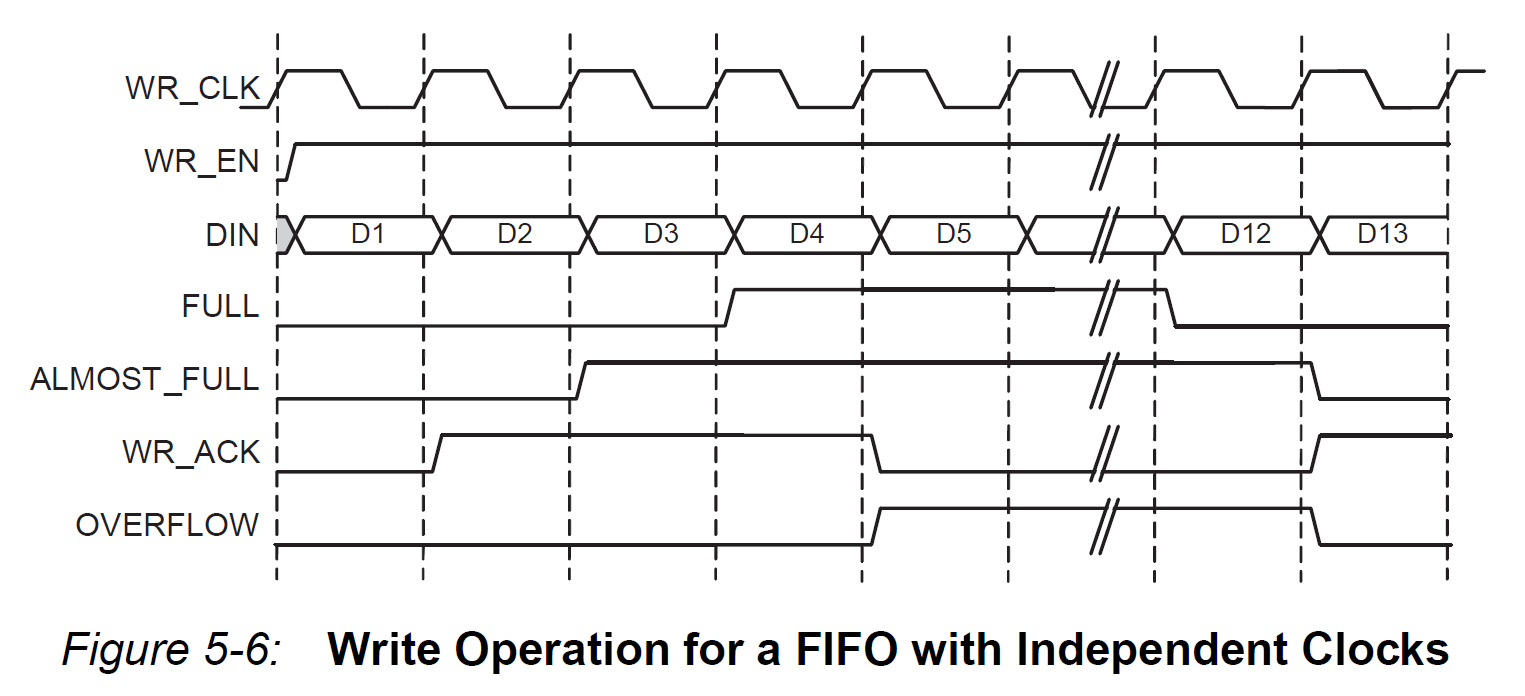
\includegraphics[width=\linewidth]{sync_fifo_write_operation.png}
	\endminipage\hfill
	\minipage{0.48\textwidth}
	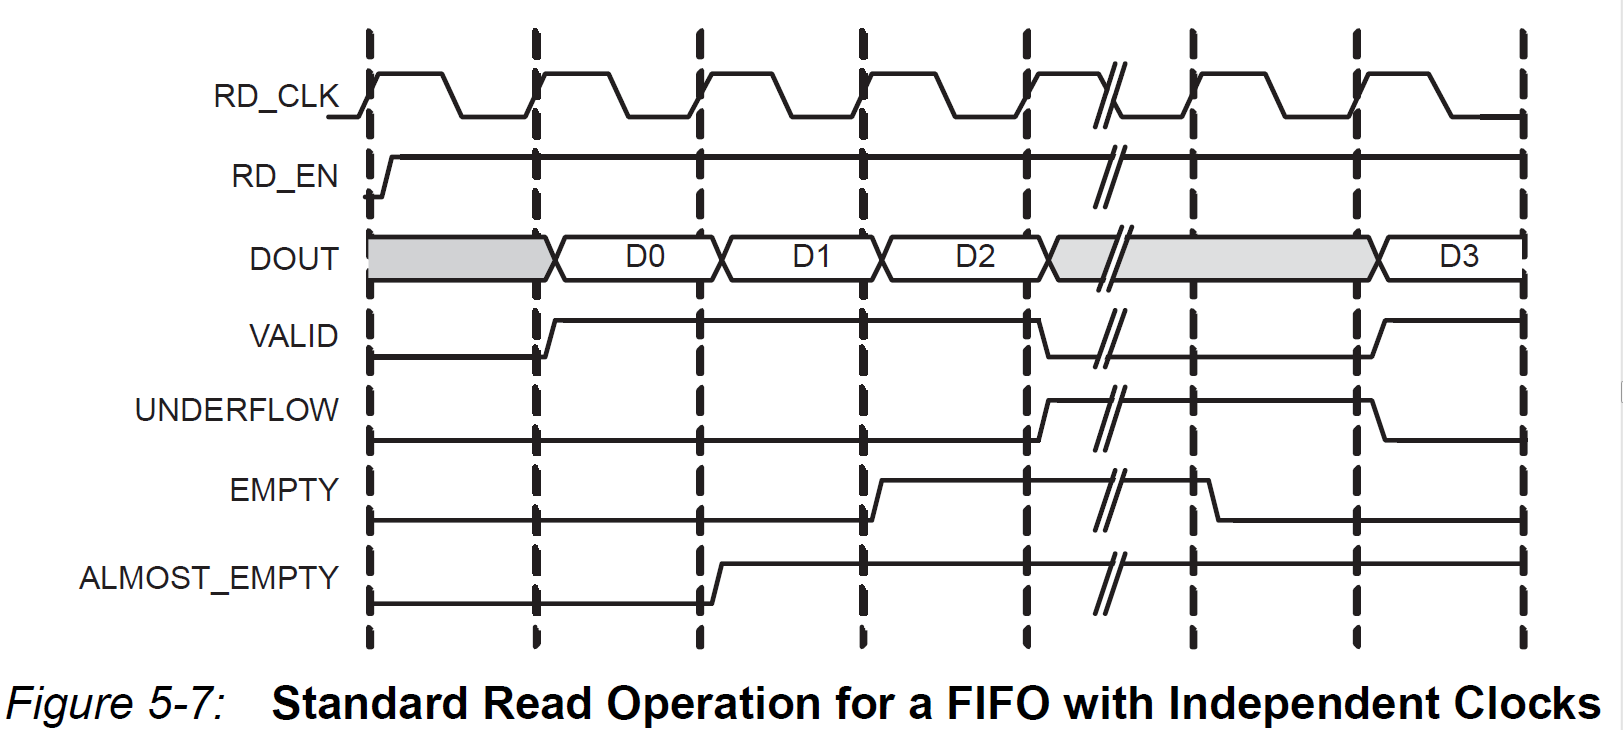
\includegraphics[width=\linewidth]{sync_fifo_read_operation.png}
	\endminipage
\end{figure}

Your FIFO doesn't need to support the \verb|ALMOST_FULL|, \verb|WR_ACK|, or \verb|OVERFLOW| signals on the write interface and it doesn't need to support the \verb|VALID|, \verb|UNDERFLOW|, or \verb|ALMOST_EMPTY| signals on the read interface.

\subsection{FIFO Testing}
We have provided a testbench for your synchronous FIFO which can be found in \verb|src/fifo_testbench.v|. This testbench can test either the synchronous or the asynchronous FIFO you will create later in the project. To change which DUT is tested, comment out or reenable the defines at the top of the testbench (\verb|SYNC_FIFO_TEST|, \verb|ASYNC_FIFO_TEST|).

The testbench we have provided performs the following test sequence, which you should understand well.
\begin{enumerate}
	\item Checks initial conditions after reset (FIFO not full and is empty)
	\item Generates random data which will be used for testing
	\item Pushes the data into the FIFO, and checks at every step that the FIFO is no longer empty
	\item When the last piece of data has been pushed into the FIFO, it checks that the FIFO is not empty and is full
	\item Verifies that cycling the clock and trying to overflow the FIFO doesn't cause any corruption of data or corruption of the full and empty flags
	\item Reads the data from the FIFO, and checks at every step that the FIFO is no longer full
	\item When the last piece of data has been read from the FIFO, it checks that the FIFO is not full and is empty
	\item Verifies that cycling the clock and trying to underflow the FIFO doesn't cause any corruption of data or corruption of the full and empty flags
	\item Checks that the data read from the FIFO matches the data that was originally written to the FIFO
	\item Prints out test debug info
\end{enumerate}

This testbench tests one particular way of interfacing with the FIFO. Of course, it is not comprehensive, and there are conditions and access patterns it does not test. We recommend adding some more tests to this testbench to verify your FIFO performs as expected. Here are a few tests to try:

\begin{itemize}
	\item Several times in a row, write to, then read from the FIFO with no clock cycle delays. This will test the FIFO in a way that it's likely to be used when buffering user I/O.
	\item Try writing and reading from the FIFO on the same cycle. This will require you to use fork/join to run two threads in parallel. Make sure that no data gets corrupted.
\end{itemize}

\section{Asynchronous FIFOs, Multi-bit Clock Crossing}
In a previous lab, we built a single-bit synchronizer, which brought an asynchronous signal from off the FPGA (buttons, rotary encoder signals) into the system clock domain. The synchronizer consisted of two D flip-flops connected in series, clocked by the system clock. This synchronizer however only works for a single bit. To synchronize an entire bus across clock domains requires a more complex synchronization scheme.

One solution, among others, is an asynchronous FIFO which works like a synchronous FIFO, except for the fact that the read and write interfaces are clocked by different clocks (with no known phase or frequency relation).

For this lab, we want to allow communication between our AC97 controller and the piano FSM. These parts operate in different clock domains (12.288 Mhz and 33 Mhz), so we need a synchronization element to safely transfer data between them.

\subsection{Async FIFO Construction}
An asynchronous FIFO is constructed similarly to a synchronous FIFO with a two ported RAM, a read and write pointer, and some logic to generate the full and empty signals. One difference is that the two ported RAM has two independently clocked ports. Another difference is that the read and write pointers need to be properly transferred to the other clock domain before going through the full and empty signal generation logic. Here is an overview of the internals of an async FIFO from the Xilinx FIFO IP Manual, page 100.

\begin{center}
	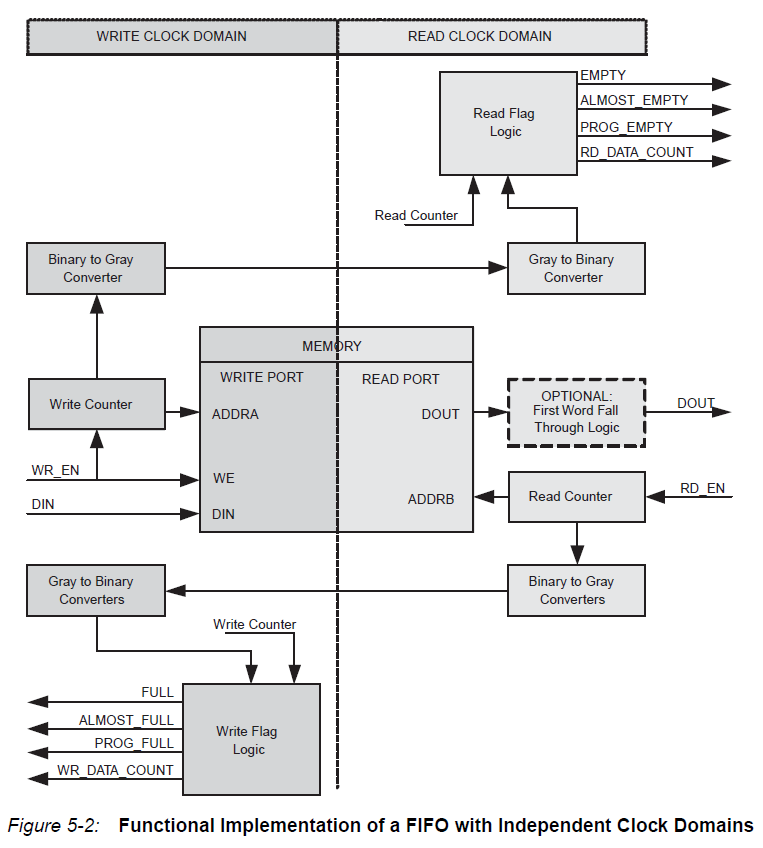
\includegraphics[height=13cm]{async_fifo_diagram.png}
\end{center}

Notice that there is a clear divide between the two different clock domains. The two arrows that cross the clock domain are the gray-coded write and read pointers. This clock domain crossing should be performed by using 2 registers in series clocked by the other clock domain, just like the 1-bit synchronizer. This will provide a robust clock crossing to avoid data corruption.

This means that the binary write pointer should be converted to a gray-coded write pointer, before passing through 2 registers in series clocked by the read clock. Then, the gray-coded write pointer has been successfully moved to the read clock domain, where it can be converted back to binary and compared against the read pointer for generating the \verb|empty| signal. The same logic chain applies to the read pointer transfer into the write clock domain.

As your build the async FIFO, you might find it useful to create binary to gray and gray to binary modules that you can instantiate in your design. The \href{https://en.wikipedia.org/wiki/Gray_code}{gray code Wikipedia article} has some psuedocode that can help you write these modules in the 'Converting to and from Gray code' section. You can make the assumption that the async FIFO for this lab and coming project will not have read and write pointers greater than 16 bits, and can design your gray code converters appropriately.

\subsection{Async FIFO Reset Behavior}
Handling resets in an async FIFO is tricky since a synchronous reset from one clock domain won't necessarily be an appropriate reset for the other clock domain. Here are a couple reset strategies:

\begin{itemize}
	\item Use one synchronous reset signal with respect to one clock domain, and propagate the reset to the other clock domain internally with a 1-bit synchronizer.
	\item Use two reset signals, one for each clock domain, and have each reset be synchronous to its respective clock.
	\item Use one global asynchronous reset signal to reset both clock domains at once.
	\item Don't use an explicit external reset signal but define initial reg values which can be synthesized for an FPGA.
\end{itemize}

For this lab, we are going to go with the last option as it is the most robust for our target (an FPGA and a temperamental AC97 bit clock). This means that you should initialize any \verb|reg| nets that represent actual registers in your async FIFO design.

\subsection{Async FIFO Interface}
The interface of the async FIFO template in \verb|hardware/src/async_fifo.v| is identical to the interface of the synchronous FIFO with the exception of having an independent read and write clock.

\subsection{Async FIFO Timing}
The timing of the async FIFO is similar to that of the synchronous FIFO with the exception that the full and empty signals can have 'delayed' transitions (of a few clock cycles) due to the need to synchronize the read and write pointers. Refer to page 110 of the \href{https://www.xilinx.com/support/documentation/ip_documentation/fifo_generator_ug175.pdf}{Xilinx FIFO IP Manual} for the timing diagrams.

\subsection{Async FIFO Testing}
The same testbench used for testing the synchronous FIFO can be used to test the async FIFO at \verb|hardware/src/fifo_testbench.v|. The only change is that at the top of the testbench file, uncomment the \verb|ASYNC_FIFO_TEST| define and comment out the \verb|SYNC_FIFO_TEST| define. Then run the testbench as usual with \verb|make sim|.

The same additional tests recommended with the synchronous FIFO are recommended for this FIFO as well. These additional tests are even more important to get right with the asynchronous FIFO, so we highly recommend writing them.

By now, you should have a working async FIFO, at least in simulation. As you may discover, basic functional simulation isn't usually a good way of telling whether a clock crossing works as expected, although it will confirm that your logic is sound.

\section{Conclusion + Checkoff}
You are done with lab 6! Please write down any and all feedback and criticism of this lab and share it with the TA. This is a brand new lab and we welcome everyone's input so that it can be improved.


\subsection{Checkoff Tasks}


\end{document}